\section{Développement du logiciel}
\subsection{Objets}
Afin de faciliter la flexibilité et l'extensibilité du code, une programmation orientée objet a été choisi (\cf \autoref{fig:diag_classe})
\begin{figure}[ht]
    \centering
    \includegraphics[width=\linewidth]{assets/figures/Diagramme_classe.drawio}
    \caption{Diagramme de classe}
    \label{fig:diag_classe}
\end{figure}
\subsection{Optimisateur}
Pour l'optimisateur, celui-ci suit le diagramme de flux (cf. \autoref{fig:algorithme_solver}) avec à la suite, un traitement des données récoltées.
\begin{figure}
    \centering
    \includegraphics[width=0.8\linewidth]{assets/figures/Diagramme_flux_opt.drawio}
    \caption{Diagramme de flux de l'optimisateur implémenté}
    \label{fig:algorithme_solver}
\end{figure}
L'utilisation de SCIP\footcite{SCIP} (qui permettra de ne pas implémenter chaque algorithme indépendamment) à travers le \gls{wrapper} or-tools\footcite{ORTOOLS} sera utilisé afin de faciliter l'intégration en python.

\section{Tests de validation et calibrage du matériel}
\subsection{Tests unitaires}
Les tests unitaires des classes et de l'optimisateur se font avec les modules \og pytest \fg (cf. \autoref{ann:test_unitaire}) et \og \textit{Coverage} \fg. Ce dernier permet de connaître le pourcentage de lignes de code testées ($94~\%$ dans ce cas (cf. \autoref{fig:coverage_global})).
\begin{figure}[H]
    \centering
    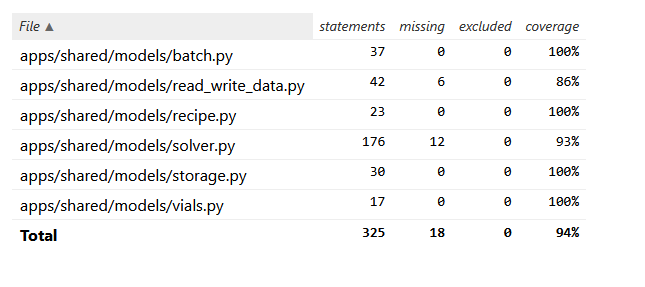
\includegraphics[width=1\linewidth]{assets/figures/coverage.png}
    \caption{Couverture du code par les tests unitaires}
    \label{fig:coverage_global}
\end{figure}
Pour le robot, les tests se sont fait en lançant les programmes et en vérifiant visuellement que le comportement soit correct. 